\documentclass[12pt]{report}

%\usepackage[a4paper, left = 2.5cm, top = 2.5cm, bottom = 2cm, right = 2cm]{geometry}

\usepackage{vmargin}

\setpapersize{A4}
\setmargins{2.5cm}       % margen izquierdo
{2.5cm}                  % margen superior
{16.5cm}                 % anchura del texto
{23.42cm}                % altura del texto
{10pt}                   % altura de los encabezados
{1cm}                    % espacio entre el texto y los encabezados
{0pt}                    % altura del pie de página
{2cm}                    % espacio entre el texto y el pie de página



\usepackage[spanish,es-tabla]{babel} % Idioma español con tablas
\usepackage{longtable}     % Usado para diseñar grandes tablas.
\usepackage{multirow} % para las tablas

\usepackage{amsmath, amssymb, amsfonts, latexsym, anyfontsize}
\usepackage{color, alltt, times}
\setcounter{secnumdepth}{3} %para que ponga 1.1.1.1 en subsubsecciones
\setcounter{tocdepth}{3}    % para que ponga subsubsecciones en el indice
\usepackage{setspace}       % Usado para %\onehalfspace  \doublespacing  \singlespace
\usepackage{booktabs}       % Para formar tablas
\usepackage{appendix}       % para los anexos
\usepackage{url}            % para citar las urls
\usepackage{pdfpages}       % para insertar documentos de tipo PDF en latex
\usepackage{epstopdf}       % para insertar imagenes en formato eps obtenidas en Matlab
\usepackage{graphicx}       % para las imagenes y gráficos
\usepackage{subfigure}      % para subfiguras

\usepackage[utf8]{inputenc}         % Para escribir en castellano
\usepackage[T1]{fontenc}

\usepackage{algorithmic}
\usepackage{algorithm}
\floatname{algorithm}{Algoritmo}
\renewcommand{\listalgorithmname}{Lista de algoritmos}
\renewcommand{\algorithmicrequire}{\textbf{Entrada:}}
\renewcommand{\algorithmicensure}{\textbf{Salida:}}
\renewcommand{\algorithmicend}{\textbf{FIN}}
\renewcommand{\algorithmicif}{\textbf{SI}}
\renewcommand{\algorithmicthen}{\textbf{ENTONCES}}
\renewcommand{\algorithmicelse}{\textbf{CASO CONTRARIO}}
\renewcommand{\algorithmicelsif}{\algorithmicelse,\ \algorithmicif}
\renewcommand{\algorithmicendif}{\algorithmicend\ \algorithmicif}
\renewcommand{\algorithmicfor}{\textbf{PARA}}
\renewcommand{\algorithmicforall}{\textbf{para todo}}
\renewcommand{\algorithmicdo}{\textbf{HACER}}
\renewcommand{\algorithmicendfor}{\algorithmicend\ \algorithmicfor}
\renewcommand{\algorithmicwhile}{\textbf{MIENTRAS}}
\renewcommand{\algorithmicendwhile}{\algorithmicend\ \algorithmicwhile}
\renewcommand{\algorithmicloop}{\textbf{REPETIR}}
\renewcommand{\algorithmicendloop}{\algorithmicend\ \algorithmicloop}
\renewcommand{\algorithmicrepeat}{\textbf{REPETIR}}
\renewcommand{\algorithmicuntil}{\textbf{HASTA}}
\renewcommand{\algorithmicprint}{\textbf{imprimir}} 
\renewcommand{\algorithmicreturn}{\textbf{RETORNAR}} 
\renewcommand{\algorithmictrue}{\textbf{cierto }} 
\renewcommand{\algorithmicfalse}{\textbf{falso }} 
 % mi archivo de traducción

\usepackage[x11names,table]{xcolor}

\usepackage{tikz,tkz-tab, tcolorbox}

\usepackage[round]{natbib} 
 
 
\begin{document}

\baselineskip 1cm
\pagestyle{plain}
%Variables
\def \authorOne {BALTODANO BELTRÁN, Massiel Estela}
\def \authorTwo {SIAPO RODRÍGUEZ, José Luis Octavio}
\def \assessor {PERALTA LUJÁN, José Luis}
\def \titleTesis {Obtención de rasgos de personalidad a partir de evaluación parcial del test de Machover en imágenes realizadas por alumnos mayores de 12 años}

%%%%%%%%%%%%%%%%%%%%%%%%%%%%% CARATULA%%%%%%%%%%%%%%%%%%%%%%%%
\textheight 19cm
\pagestyle{empty}
\begin{center}
 {\bf {\fontsize{14}{16.8}\selectfont UNIVERSIDAD NACIONAL DE TRUJILLO}}     
 
    {\bf{\fontsize{14}{16.8}\selectfont Facultad de Ciencias Físicas y Matemáticas}} 

  {\bf{\fontsize{14}{16.8}\selectfont Escuela Profesional de Informática}}
\end{center}  

\begin{figure}[ht]
\begin{center}

\includegraphics[width=.4\textwidth]{images/unt}
\end{center}
\end{figure}
\vskip 0.5cm

\begin{center}
  {\bf\Large{{\fontsize{17}{20.4}\selectfont{\titleTesis} }}}     
\end{center}
\vskip 0.5cm

\begin{center}
{\Large{TESIS}}
\end{center}
\begin{center}
{\large{\hspace*{0.4cm} PARA OPTAR EL TÍTULO PROFESIONAL DE INGENIERO  INFORMÁTICO}}
\end{center}

\vskip 0.6cm
\begin{center}
  { \fontsize{14}{16.8}\selectfont {\hspace{-2.9cm}AUTOR(ES): \authorOne}} \\
    { \fontsize{14}{16.8}\selectfont {\hspace{-0.4cm} \authorTwo}}\\
    \vskip 0.2cm
    { \fontsize{14}{16.8}\selectfont {\hspace{-1.7cm} ASESOR: \assessor}}

     
\end{center}   


\vskip 1.1cm
\begin{center}    
{\bf {\fontsize{14}{16.8}\selectfont TRUJILLO - PERÚ
\vskip 0.0cm
\hspace*{-0.2cm} 
2019 }}
\end{center} 
\newpage
%%%%%%%%%%%%%%%%%%%%%%%%%%%%%%%%%%%%%%%%%%%%%%%%%%%%%%%%%%%%%%%%%%%%%%%%%%%


%%%%%%%%%%%%%%%%%%%%%%%%%%%%CONTRA CARATULA 1 %%%%%%%%%%%%%%%%%%%%%%%%%%%%%
%\newpage
%\pagestyle{plain}
%\pagenumbering{roman}

%\hspace*{6cm}
%\vskip 9cm
%\begin{center}
%   {\bf \doublespacing {\fontsize{17}{20.4}\selectfont{MODELO PARA LA RUTERIZACIÓN }}}     
%\end{center} 
%\newpage
%%%%%%%%%%%%%%%%%%%%%%%%%%%%%%%%%%%%%%%%%%%%%%%%%%%%%%%%%%%%%%%%%%%%%%%%%%%


%%%%%%%%%%%%%%%%%%%%%%%%%%%%% CONTRA CARATULA 2 %%%%%%%%%%%%%%%%%%%%%%%
%\begin{center}
%   {\bf {\fontsize{14}{16.8}\selectfont{EDGAR PECHE PERLADO}}}\\    
%      {\bf {\fontsize{14}{16.8}\selectfont{MANUEL PEREZ YON}}}       
%   \end{center}   

%\vskip 3.2cm
%\begin{center}
%   {\bf \doublespacing {\fontsize{17}{20.4}\selectfont{MODELO PARA LA RUTERIZACIÓN }}}     
%\end{center}   
%  \vskip 2cm
%\begin{verse}
% \fontsize{12}{14.4}\selectfont{\hspace*{0.6cm}Tesis presentada a la Escuela Profesional de Informática en la Facultad de Ciencias Físicas y Matemáticas de la Universidad Nacional de Trujillo, como requisito parcial para la obtención del grado de Bachiller en ciencia de la computación ( Título profesional de Ing. Informático)}
%\end{verse}

%\vskip 1.5cm 
%{\fontsize{14}{16.8}\selectfont ASESOR: JOSÉ A. RODRIGUEZ MELQUIADES} 
% \vskip 1cm 
% \begin{center}    
% \vskip 2cm
%{\fontsize{14}{16.8}\selectfont Trujillo - Perú
%\vskip 0.2cm
%\hspace*{-0.2cm} 
%2019}
%\end{center} 
%\newpage
%%%%%%%%%%%%%%%%%%%%%%%%%%%%%%%%%%%%%%%%%%%%%%%%%%%%%%%%%%%%%%%%%%%


%%%%%%%%%%%%%%%%%%%%%%%%%%%% DEDICATORIA %%%%%%%%%%%%%%%%%%%%%%
\pagestyle{plain}
\pagenumbering{roman}
 
 \addcontentsline{toc}{chapter}{Dedicatoria}
 {\bf\Large {Dedico esta tesis a :}}
 \vskip 1cm
\begin{quotation}
{\it Mis padres ....
\vskip 1cm
Mi hermano ... .
\vskip 1cm
Mi ... .}
\end{quotation}
%%%%%%%%%%%%%%%%%%%%%%%%%%%%%%%%%%%%%%%%%%%%%%%%%%%%%%%%%%%%%%%%%%%%%%%%%%%


\newpage

 \addcontentsline{toc}{chapter}{Agradecimientos}
 {\bf\Large {\flushleft{Agradecimientos}}}
 \vskip 1.5cm
\begin{quotation}
Agradezco a Dios por haberme bendecido en toda mi vida ....
{\vskip 1cm}
A mis profesores del Departamento de Informática, de los cuales recibi una gran cantidad de conocimientos  . . .
\vskip 1cm
A mi asesor Prof. Dr. José A. Rodríguez Melquiades que siempre se mostro disponible e interesado en ayudarme.
\vskip 1cm
 . . .
 \end{quotation}
\newpage 
%%%%%%%%%%%%%%%%%%%%%%%%%%%%%%%%%%%%%%%%%%%%%%%%%%%%%%%%%%%%%%%%%%%%%%%%%%%
              % Datos de la tesis

%%%%%%%%%%%%%%%%%%%%%%%%%%%% AGRADECIMENTOS %%%%%%%%%%%%%%%%%%%%%%

%%%%%%%%%%%%%%%%%%%%   ACTA SUSTENTACION   %%%%%%%%%%%%%%%%%%%%%%%%

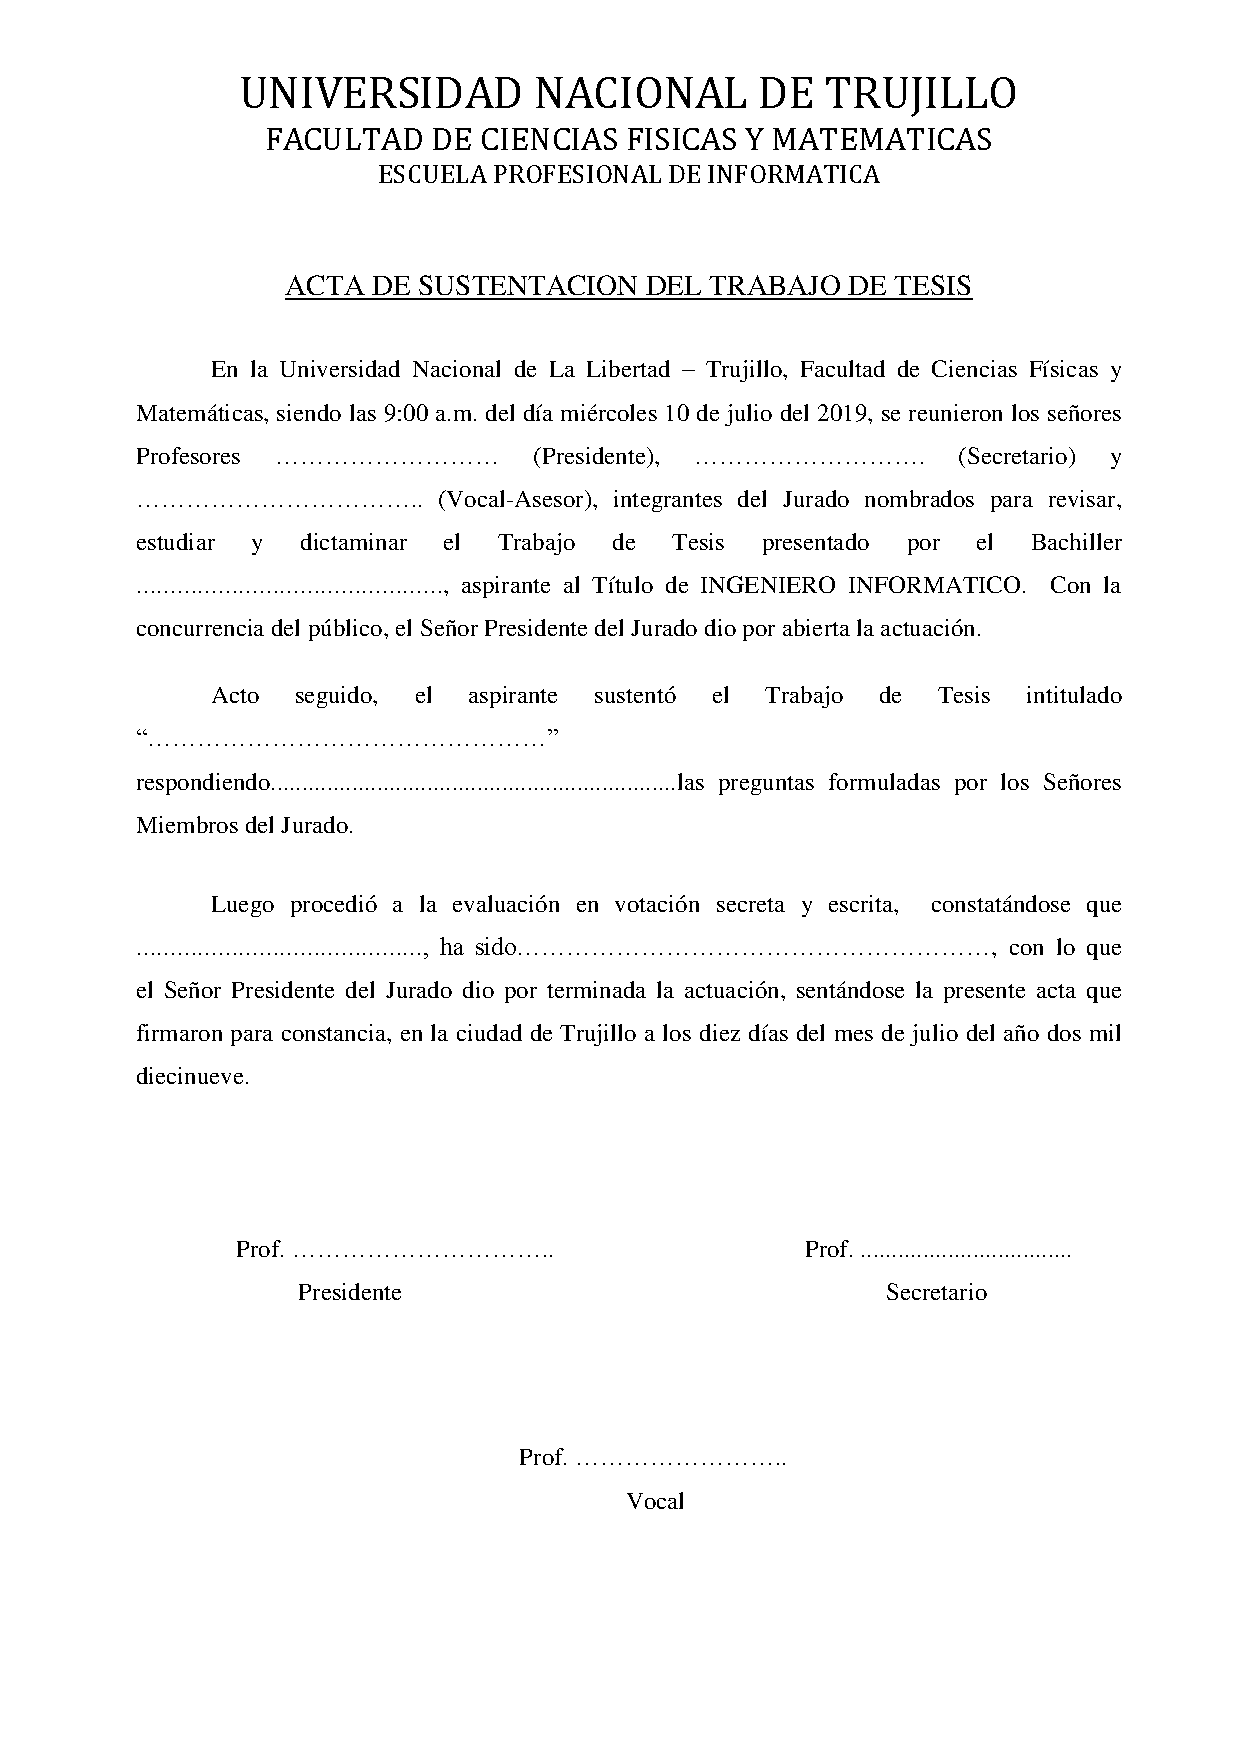
\includepdf[pagecommand={}]{Acta_Sustentacion.pdf}


%%%%%%%%%%%%%%%%%%%%%%%%%%%%%%%%%%%%%%%%%%%%%%%%%%%%%%%%%%%%%%%%%%%

%%%%%%%%%%%%%%%%%%%%%%%%%%%% RESUMEN%%%%%%%%%%%%%%%%%%%%%%
\newpage
\begin{center}
 \addcontentsline{toc}{chapter}{Resumen}
 {\bf\LARGE Resumen}
\end{center} 
\vskip 0.5cm
\begin{quotation}
{\bf Ejemplo:}\par

La investigación bibliográfica revela una preocupación de los gobiernos en lo relacionado al destino final de los residuos sólidos urbanos (RSU), con el objetivo de preservar la salud de la población, el medio ambiente urbano y rural. En este contexto y para el caso de las ciudades peruanas se esperaba que con la desactivación legal de los botaderos hasta el año 2020, surgiesen medidas que viabilicen la colecta selectiva, reciclaje y reutilización para aproximadamente el $80\%$ del volumen total de residuos colectados y destinados a locales no apropiados. 
\vskip 0.2cm 
En este sentido esta investigación tiene como objetivo principal modelar y planificar una red de logística reversa para una región urbana, dimensionando el flujo de RSU que será movido a lo largo de la red, el número y capacidad de las estaciones de colecta, de las unidades productivas y especiales necesarias para su colecta, transporte y disposición final. Los resultados muestran que es posible realizar un modelo matemático para este tipo de problemas, así como su aplicación en diversas regiones sin necesidad de grandes cambios en el modelo propuesto.    

\vskip 0.3cm
\hspace*{-0.6cm}{\bf Palabras claves:} residuos sólidos urbanos, logística reversa, modelo matemático.
\end{quotation}
%%%%%%%%%%%%%%%%%%%%%%%%%%%%%%%%%%%%%%%%%%%%%%%%%%%%%%%%%%%%%%%%%%%%%%%%%%%%%%%%%%%%


%%%%%%%%%%%%%%%%%%%%%%%%%%%%ABSTRACT%%%%%%%%%%%%%%%%%%%%%%
\newpage
\begin{center}
 \addcontentsline{toc}{chapter}{Abstract}
 {\bf\LARGE Abstract}\vskip 1.5cm
\end{center} 
\begin{quotation}

{\bf Ejemplo:}\par

The literature reveals a concern of Governments with the disposal of municipal solid waste (MSW) in order to preserve the health of the population, the urban and rural environment. In this context and for the case of peruvian cities, it was expected that, with the legal command for the deactivation of landfills by 2020, measures would be adopted in order to enable the selective collection, recycling and reuse for about $80\%$ of the total volume of collected solid waste and intended to inappropriate places. 
\vskip 0.2cm
In this sense, this research aims to model and plan a reverse logistics network to an urban area, dimensioning the flow of MSW that will be moved along the network, the number and capacity of collection stations, and the productive and special units required for their collection, transportation and final disposal. The results show to be possible perform mathematical modeling of this problem with low investment, as well as apply it in various regions without major changes in the proposed model.

\vskip 0.3cm
\hspace*{-0.6cm}{\bf Keywords:} solid waste, reverse logistics, mathematical modeling.
\end{quotation}
%%%%%%%%%%%%%%%%%%%%%%%%%%%%%%%%%%%%%%%%%%%%%%%%%%%%%%%%%%%%%%%%%%%%%%%%%%%%%%


%%%%%%%%%%%%%%%%%%%%%%%%%%% LISTA DE SIMBOLOS %%%%%%%%%%%%%%%%%%%%%%
\newpage
\addcontentsline{toc}{chapter}{Lista de símbolos}
 {\bf\LARGE Lista de símbolos}
 \vskip 1.5cm
Constantes: 
\begin{enumerate}
\item[(1)]$r,\overline{r} $ \hspace*{0.8cm} Indice que denota regiones.
\item[(2)] $n $ \hspace*{1.1cm} Indice de bienes finales deseados por los consumidores.
\item[(3)] ...
\vskip 3cm
\end{enumerate} 
\vskip 0.3cm
Variables:
\begin{enumerate}
\item[(5)] $ x^{r} $ \hspace*{1cm} Vector columna que denota la actividad de producción.
\item[(6)] $ u^{r} $ \hspace*{1.2cm} . . .
\end{enumerate}

              % Datos de la tesis
\listoffigures               % indice de figuras
\addcontentsline{toc}{chapter}{Índice de Figuras}
\listoftables                % indice de tablas
\addcontentsline{toc}{chapter}{Índice de Tablas}
\tableofcontents             % indice de materias
\chapter{Introducción}
\pagenumbering{arabic}
\setcounter{page}{1}
%\renewcommand{\baselinestretch}{2} %doble espacio paratodo el texto
%\renewcommand{\baselinestretch }{1.5}
 


{\bf Ejemplo:}\par

A medida que las ciudades crecían, el propio sistema urbano como un todo iba quedando cada vez más complejo e insuficiente para atender la fuerte demanda de la población por servicios urbanos. Las instituciones responsables por la oferta de tales servicios urbanos no han podido acompañar el ritmo de crecimiento de las demandas, ya que necesitan inversiones para ampliar los servicios de proyectos innovadores que se adapten a la nueva realidad de la sociedad moderna y de modelos de gestión más eficientes y eficaces que dinamicen la toma de decisiones, así como una participación más proactiva de la comunidad y de todos los actores involucrados de forma directa e indirecta en esos servicios.   
\vskip 0.3cm
El transporte de carga tiene cierta ventaja sobre el transporte de personas, pues es posible intervenir e influir en los flujos de los viajes a través  de una buena administración de los horarios de los sistemas logísticos de entrega, y colecta de las empresas y por medio de la implementación de proyectos de logística urbana y definición de políticas de transporte de carga por parte de los gobiernos locales, en sociedad con las empresas transportadoras y la comunidad. Diversos proyectos se han aplicado con bastante éxito en varias ciudades del primer mundo \citep{Santos}, trayendo ganancias a todos los actores y una reducción significativa de los impactos negativos en los principales centros urbanos.    

\section{Justificación de la investigación}
La mayoría de las investigaciones se efectúan con un propósito definido. Tal propósito debe ser lo suficientemente fuerte para que justifique su realización. \cite{Erica}  

\begin{enumerate}
\item[(a)] Razones o motivos e importancia del tema a ser investigado. 
\item[(b)]Sustentar la pertinencia de la pregunta o problema que se abordará en la investigación.
\item[(c)]Considerar los resultados esperados e impactos previstos.
\end{enumerate}



{\bf Ejemplo:}\par

De esta forma, los sistemas integrados para el manejo, tratamiento y disposición final de los RSU que ya existen en diversas ciudades y capitales de los países desarrollados, se hacen referencias para la investigación y justifican posibles adaptaciones para la realidad peruana con el objetivo de que las ciudades sean ambientes más sustentables y competitivos.
\vskip 0.3cm
 Por lo tanto, se puede concluir que realmente existe una necesidad para planificar y modelar una red logística reversa que atienda a las necesidades de una región urbana y que contribuya con la adecuada disposición de los residuos urbanos. A partir del modelamiento es posible estructurar el sistema organizacional, gerencial, operacional y de información de toda la red  de logística reversa, y todas las otras acciones.


\section{Formulación del problema}
Plantear el problema no es otra cosa mas que afinar y estructurar formalmente la idea de investigación. El planteamiento del problema puede ser sencillo o complejo dependiendo de la familiarización del investigador en el tema a tratar.\par    
\vskip 0.3cm
Los criterios para formular un problema de investigación son:
\begin{enumerate}
\item[a)] El problema debe ser formulado claramente y sin ambiguedad como pregunta: ¿Qué efecto?; ¿en qué condiciones ...?; ¿cuál es la probabilidad de ...?; ¿cómo se relaciona ... con ...?; ¿cómo ...?.
\vskip 0.3cm
\item[b)] El planteamiento debe implicar la posibilidad de realizar una prueba empírica o una recolección de datos, es decir, la factibilidad de observarse en la realidad o en un entorno. 
\end{enumerate}
Por lo tanto, los elementos para plantear un problema de investigación son tres y estan relacionados entre si: Los objetivos que persigue la investigación; las preguntas de investigación y la justificación del estudio. \cite{Erica}
\vskip 0.3cm

{\bf Ejemplo:}\par

  En este trabajo, se propone discutir el modelo de red  de logística reversa basado en el problema del ruteo de vehículos para responder a la siguiente pregunta:
 \begin{center} 
     ?`Cómo viabilizar una red logística reversa en regiones urbanas minimizando los costos logísticos de ruteo y transporte de los RSU hasta su disposición final?
 \end{center}


\section{Hipótesis}
Preferentemente para investigaciones explicativas debe ser una respuesta a priori y tentativa guardando coherencia con el problema científico, se formula como una proposición afirmativa, con un lenguaje claro y específico.  Las hipótesis se obtienen por deducción lógica y está sustentada en los conocimientos científicos. \par  
\vskip 0.3cm
{\bf Criterios para formular hipótesis:} \cite{Erica}
\begin{enumerate}
\item[a)] Toda hipótesis de investigación debe ser verificable estadísticamente.  Puede ser difícil o imposible de verificar porque no existe un conocimiento sobre el cual se pueda formular una hipótesis, o bien, porque una o más variables no son medibles.
\vskip 0.2cm
\item[b)] Toda hipótesis debe indicar la relación entre variables, lo que implica que las variables deben ser medibles.
\vskip 0.2cm
\item[c)] Toda hipótesis debe tener sus límites. Pueden escogerse hipótesis que sean sencillas de validar, y sin embargo, altamente significativas.
\vskip 0.2cm
\item[d)] El investigador debe tener una razón específica para considerar una hipótesis, ya sea teórica o por alguna evidencia concreta.    
\end{enumerate}





\section{Objetivos}
Es necesario establecer qué pretende la investigación, es decir, cuáles son sus objetivos. Hay investigaciones que buscan contribuir a resolver un problema en especial, y otras tienen como objetivo principal probar una teoría o aportar evidencia empírica en favor de ella. \par 
\vskip 0.3cm
Segun \cite{Rojas}, los objetivos tienen que expresarse con claridad para evitar posibles desviaciones en el proceso de investigación y deben ser susceptibles de alcanzarse; son las guías del estudio y hay que tenerlos presentes durante todo su desarrollo. Los objetivos deben ser congruentes entre sí.
\vskip 0.3cm
Describir el objetivo central o propósito del proyecto de investigación (debe estar alineado con el problema e hipótesis), así como los objetivos específicos, los cuales deben reflejar los cambios que se esperan lograr en trabajo de tesis (variables). Para estos objetivos específicos utilice verbos como: describir, indicar, modificar, controlar, producir (tecnologías), recuperar, etc..

\subsection{Generales}
Debe explicitar lo que se espera lograr con el estudio en términos de conocimiento. Debe dar una noción clara de lo que se pretende describir, determinar, identificar, comparar y verificar.


\subsection{Específicos}
Son la descomposición y secuencia lógica del objetivo general. Son un anticipo del diseño de la investigación.
\vskip 0.3cm



{\bf Ejemplo de objetivos:}\\
{\bf Objetivo General:}
\begin{enumerate}
\item[a)] La investigación tiene como objetivo principal modelar y planificar una red logística reversa para una región urbana, dimensionando el flujo de RSU que será transportado a lo largo de la red y determinar el número y capacidad de las estaciones de colecta y de la unidades productivas y especiales necesarias para la atención de la región, en cuanto a la colecta, transporte y disposición final de los RSU.
\vskip 0.3cm
\item[b)]Con la optimización del modelo de colecta de RSU, es posible reorganizar el sistema logístico reverso de una ciudad de forma que se consiga un mejor dimensionamiento de la red, con la consecuente disminución del número que circulan en la ciudad.
\end{enumerate}
\vskip 0.2cm
{\bf Objetivos específicos:}
\begin{enumerate}
\item[a)] Aplicar una metodología de programación lineal entera, considerada computacionalmente como un problema que pertenece a la clase de complejidad NP \citep{Korte} para solucionar el problema.
\item[b)] Implementar con CPLEX, rodando en el sistema operativo Linux, los modelos propuestos, validarlos y testarlos en un caso práctico.
\end{enumerate}




\section{Estructura de la tesis}

{\bf Ejemplo:}\par
\vskip 0.1cm
El presente trabajo está dividido en cinco capítulos. El primer capítulo presenta los aspectos generales de la investigación realizada tal como justificación, formulación del problema, hipótesis, los objetivos y la estructura de la tesis.

En el capítulo dos se presenta el referencial teórico, soporte del tema, contemplando los conceptos de sustentabilidad urbana, logística directa y reversa, modelamiento y ruteo. Finalmente el método empleado en la investigación.

El tercer capítulo trata del tema central de la tesis, diseñandose los modelos respectivos propuestos...   

 En el cuarto capítulo se presentan los resultados y discusión obtenida en la investigación. En el capítulo cinco se presentan las consideraciones finales obtenidas en esta tesis. Inicialmente se presentan las conclusiones, seguida de las recomendaciones para futuras investigaciones relacionadas al tema en cuestión.

Finalmente las referencias bibliográficas usadas para la investigación en esta tesis y los anexos donde se presentan los programas elaborados y en apéndice un pequeño glosario de ciertos términos usados en esta investigación. Finalmente la declaración jurada y autorización de la tesis.




\chapter{Materiales y métodos}

{\bf Ejemplo:}\par

En este capítulo se explica cual fue la metodología empleada para la solución del problema formulado, además de una reseña del material bibliográfico investigado con relación a los temas considerados en esta investigación. Los conocimientos investigados son muy amplios, principalmente aquel que ayudó a consolidar las bases del conocimiento científico para elaborar esta tesis, como lo son los temas de optimización combinatoria, complejidad computacional, metaheurísticas, ciencia de la información y logística, conocimientos sin los cuales sería difícil de modelar y solucionar matemática y computacionalmente cualquier tipo de problema de optimización.
%\vskip 1cm 


\section{Marco teórico}
\subsection{Optimización combinatoria y complejidad computacional}
\subsubsection{Problemas combinatorios}
\subsubsection{Heurísticas y metaheurísticas}

\subsection{Sustentabilidad}

{\bf Ejemplo:}\par

La configuración, característica, jurisdicción administrativa, relaciones económicas, sociales y ambientales de un espacio urbano se define por la población y por la función que ella desarrolla en un área geográfica o región \citep{Bugliarello}. De este modo las ciudades son sistemas dinámicos que interactúan continua y constantemente con su medio ambiente, acompañando las características, perfil, cultura y ritmo de desarrollo económico y social de su población. Los medios de transporte juegan un papel importante en tal ritmo de desarrollo de las ciudades, ya que ellos tienen como función relacional los factores poblacionales con los factores uso del suelo.  
\vskip 1cm
El desarrollo sustentable, (Figura 2.1), estará garantizado si se consideran tres aspectos fundamentales: económico, social y ambiental, donde la intersección de estos aspectos garantiza la calidad de vida en el espacio urbano y el equilibrio en las clases sociales en busca del bienestar \citep{Tanguay}.

\begin{figure}[ht]
\begin{center}
% \includegraphics[width=0.3\textwidth]{Figura2}
\end{center}
\begin{center}
\vskip -0.5cm
\caption{\small{Aspectos claves para el desarrollo sustentable.}}
{\small{Fuente: \cite{Tanguay}}}
\end{center}
\end{figure}

\subsection{Logística directa y reversa}

\subsubsection{Logística directa}

{\bf Ejemplo:}\par

\cite{Ghiani} entienden que la logística trata de la planificación y control de los flujos de materiales e informaciones relacionadas en las organizaciones, tanto en los sectores público y privado. Además su misión es hacer la entrega de los productos correctos, en el local correcto y en la hora correcta, optimizando los costos operacionales totales del proceso.
satisfaciendo un determinado conjunto de restricciones o condiciones.\par

\subsubsection{Logística reversa}

{\bf Ejemplo:}\par

En los años 90 se presentaron definiciones generales las cuales vienen siendo mejoradas. \cite{Dekker} presenta una mejora en la definición de logística reversa como  ”el proceso de planificación, implementación y control de los flujos de materias-primas, en procesos de inventarios y bienes acabados, desde el punto de fabricación, distribución o uso, hacia el punto de recuperación o de eliminación”. 
\begin{figure}[ht]
\begin{center}
% \includegraphics[width=0.3\textwidth]{Figura1}
\end{center}
\begin{center}
\vskip -0.5cm
\caption{\small{Logística reversa incluida en el desarrollo sustentable.}}
{\small{Fuente: Adaptación de \cite{Tanguay}}}
\end{center}
\end{figure}


\subsubsection{Modelos}

\subsection{Modelamiento y ruteo }

{\bf Ejemplo:}\par

El modelamiento matemático es una alternativa para expresar formalmente hechos reales que pueden ayudar en el proceso de toma de decisiones. El modelamiento permite la simulación de procesos  y de escenarios con la introducción de índices de desempeño que permitan cuantificar los costos y beneficios de la implementación del sistema, la mejoría de la sustentabilidad urbana y por supuesto los índices de contaminación en las grandes ciudades y su impacto en todo el medio ambiente. 

\subsubsection{Modelos utilizados en los problemas de ruteo de vehículo }

{\bf Ejemplo:}\par

El problema de ruteo de vehículos \citep{Ombuki, Yeun} y sus variantes han ganado mucho interés en la comunidad académica. La intención de estar más cerca a la realidad mediante el modelamiento matemático, hace que se hayan desarrollado nuevos modelos de optimización. \par
\vskip 0.2cm

\begin{table}[h!]
\begin{center}
\caption{\small{Resultados computacionales obtenidos en el modelo de \cite{Ombuki}}}
\end{center}
\vskip -0.7cm
\begin{tabular}{|c|c|c|c|c|}
\hline 
\rowcolor{LightBlue2}{\small Escenarios} & {\small Demanda cliente (ton.)} & {\small Tiempo (min.)} & {\small Costo ($\$$)} \\ 
\hline 
{\small 1} & {\small P1:1; P2:2; P3:2; P4:2; P5:1} & {\small 0.12} & {\small 667.42} \\ 
\hline 
{\small 2} & {\small P1:1; P2:2; P3:2; P4:2; P5:1; P:4; P7:3} & {\small 56.54} & {\small 1744.35} \\ 
\hline 
{\small 3} & {\small P1: 1; P2:2; P3:2; P4:2; P5:1; P6: 4; P7:3; P8:2; P9:2} & {\small 287.70} & {\small 1750.72} \\ 
\hline 
{\small 4} & {\small P1:1; P2:2; P3: 2; P4:2; P5:1; P6:4; P7:3; P8:2; P9:2; P10:1} & {\small 1848.57} & {\small 1773.46} \\ 
\hline 
{\small 5} & {\small P1:1; P2:2; P3: 2; P4:2; P5:1; P6:4; P7:3; P8:2; P9:2; P10:1} & {\small 1848.57} & {\small 1773.46} \\ 
\hline 
{\small 6} & {\small P1:1; P2:2; P3: 2; P4:2; P5:1; P6:4; P7:3; P8:2; P9:2; P10:1} & {\small 1848.57} & {\small 1773.46} \\ 
\hline 
\end{tabular} 
\begin{center}
\vskip -0.2cm
{\small{Fuente: Resultados obtenidos con CPLEX.}}
\end{center}
\end{table}



\section{Método de la investigación}
De acuerdo con \cite{Erica}, para el desarrollo del método debe presentarse un bosquejo de la manera  en que se propone llevar a cabo la investigación, es decir, el camino a seguir o los pasos a seguir para realizar una cosa. Cuando mas complejo sea el bosquejo  más fácil se desarrollará el proceso de investigación. Se utiliza el vocablo método en vez de metodología, ya este último se considera equivocado, en el sentido en que se le utiliza comúnmente en informes de investigación. 
\vskip 0.3cm
Los tipos de método a usar para TG en informática se considera:
\begin{enumerate}
\item[a)] {\bf Método deductivo:} Es un método de razonamiento que consiste en tomar conclusiones generales para explicaciones partículares. El método se inicia con el análisis de los postulados, teoremas, leyes, principios, etc., de aplicación universal y de comprobada validez, para aplicarlos  a soluciones o hechos particulares. 

\item[b)]{\bf Método cuantitativo:} Se fundamenta en la medición de las características de los fenómenos, lo cual supone derivar de un marco conceptual pertinente al problema analizado, una serie de postulados que expresen relaciones entre las variables estudiadas de forma deductiva, es decir, estudia fenómenos susceptibles de cuantificación y utiliza pruebas estadísticas para el análisis de datos. Este método tiende a generalizar y normalizar resultados. 
\end{enumerate}

Por lo tanto, plantear el objeto de estudio, el diseño de investigación a usar, las técnicas de recolección de la información a ser utilizadas, definir la población y tamaño de la muestra que debe ser representativa y necesaria para hacer generalizaciones, {\bf etapas del estudio} y análisis estadístico. El método de estudio entre otras cosas se refiere a la secuencia de pasos que se sigue para alcanzar los objetivos trazados, considerando los métodos deductivo y cuantitativo.\par




\chapter{Nombre de la propuesta o tema central de la tesis}

{\bf Ejemplo:}\par

Basado en los conceptos discutidos en los capítulos 1 y 2, así como de la experiencia obtenida del análisis de resultados de los modelos matemáticos estudiados y programados con CPLEX, se caracterizan los principales elementos que componen el modelo propuesto en este trabajo para la colecta y transporte de RSU en un área urbana. Así, se estructura una red logística reversa para los RSU considerando diferentes centros especializados o unidades  productivas para atender las diferentes fases del proceso en la red. En este proceso de modelamiento se tuvo cuidado en mantener la propuesta lo mas cerca a la realidad de las ciudades, donde el modelo fue testado y validado.

\section{Proceso de modelamiento} 

{\bf Ejemplo:}\par

La planificación y modelamiento del sistema de logística reversa de una área urbana es una fase importante y estratégica, para obtener en el futuro óptimos resultados en el proceso de gerenciamiento y operación del sistema reverso de RSU. El modelamiento permite determinar la localización de las estaciones de colecta y de unidades especiales necesarias, asi como el flujo que será movido a los largo de la red permitiendo dimensionar todo el sistema y sus componentes (Figura 3.1).
\vskip 0.3cm
\begin{figure}[ht]
\begin{center}
% \includegraphics[width=.6\textwidth]{Figura3}
\end{center}
\begin{center}
\vskip -0.5cm
\caption{\small{Esquema del proceso de colecta y transporte de RSU.}}
{\small{Fuente: Elaboración propia}}
\end{center}
\end{figure}

\subsection{Proceso de ruteo}

\begin{algorithm}
\begin{algorithmic}[htbp]
\REQUIRE NP,NV,Dij,Tij,DM,CM,P,numVecinos,numIteraciones,persistencia.  % Entrada
 \label{lin:algoritmo_pseudocodigo}
\ENSURE RUTAS.                                                          % Salida

\STATE $i \leftarrow 0 $

\STATE Inicializar lista de vecinos y la memoria tabú.
\STATE Generar solución inicial.
\STATE Evaluar solucion inicial.
\WHILE {$numIteraciones  >  i$}
\STATE Generar los vecinos.
\STATE Evaluar los vecinos.
\STATE Elegir al mejor vecino.
\IF{Mejor vecino tiene una mejor solución}
\STATE Reemplazar solución inicial y agregarlo a la memoria tabú con su persistencia respectiva.

\ELSE
\STATE Agregar mejor vecino a la memoria tabú con su persistencia respectiva.

\ENDIF
\STATE Disminuir persistencia de todos los que estan en la memoria tabú excepto del último elemento agregado.

\IF{La persistencia de los elementos llega a cero}
\STATE Retirar el elemento de la memoria tabú.
\ENDIF

\STATE $i++$
\ENDWHILE
\RETURN  La mejor solución.


\end{algorithmic}
\caption{Busca tabú}
\label{alg:algoritmoBT}
\end{algorithm}


\section{Implementación} 



\chapter{Resultados y discusión de la tesis}


Al culminar con la investigación se llegaron a resultados interesantes del punto de vista tanto teórico como computacional. Estos resultados muestran que se contrasta la hipótesis planteada durante el proceso de elaboración del plan de investigación, es decir, que se logró demostrar la relación entre las variables de estudio formuladas en la investigación.

\section{Teóricos}

\section{Computacionales}




\chapter{Consideraciones finales}


\section{Conclusiones}

{\bf Ejemplo}\\
La investigación bibliográfica revela que realmente existe una preocupación de los gobiernos con el destino final de los residuos sólidos, con el objetivo de preservar la salud de la población y el medio ambiente urbano y rural. Por ejemplo, se observa la creación de la Ley 12305. Sin embargo existe una laguna entre las metas propuestas en la ley con las metas reales de los gobiernos locales. Eso se debe a la falta de una buena estructura organizacional, gerencial y operacional de los gobiernos locales capaz de atender las demandas locales y las necesidades de la población.
\vskip 0.3cm
La falta de cuadros especializados, tanto en los gobiernos centrales como locales, para realizar la planificación y modelamiento de una red logística reversa puede ser compensada con la contribución de los investigadores que actúan en ese campo del conocimiento. Es muy difícil la formación de un equipo que tenga todo el conocimiento en las áreas de ciencia de la computación, de geo procesamiento, de modelamiento matemático y de logística reversa, entre otras. Esa es una de las principales justificativas que los gobiernos, argumentan a la falta de planificación de una red logística reversa que funciones eficaz y eficientemente. 
\vskip 0.3cm
Por lo tanto, como quedó demostrado a lo largo de este trabajo, es posible realizar el modelamiento matemático para este tipo de problema con baja inversión, así como aplicarlo en varias regiones sin necesidad de grandes cambios en el modelamiento propuesto. El modelo propuesto calcula los flujos en la red logística reversa, permitiendo dimensionar la cantidad y capacidad de las unidades productivas y de los vehículos. 
\vskip 0.3cm
...


\section{Trabajos futuros}




\cleardoublepage
\renewcommand\bibname{Referencias bibliográficas}
\addcontentsline{toc}{chapter}{ Referencias bibliográfícas}
\bibliographystyle{apalike}   % estilo de la bibliografía APA.
\bibliography{Bibliografia}   % Archivo de Bibliografia.bib.

                % Capitulos de la tesis

\appendix
\chapter{Primer apendice}
(ES OPCIONAL) 
hola como estas
\chapter{Segundo apendice}
(ES OPCIONAL)
si te escucho


\vskip 0.5cm



           % Apendice

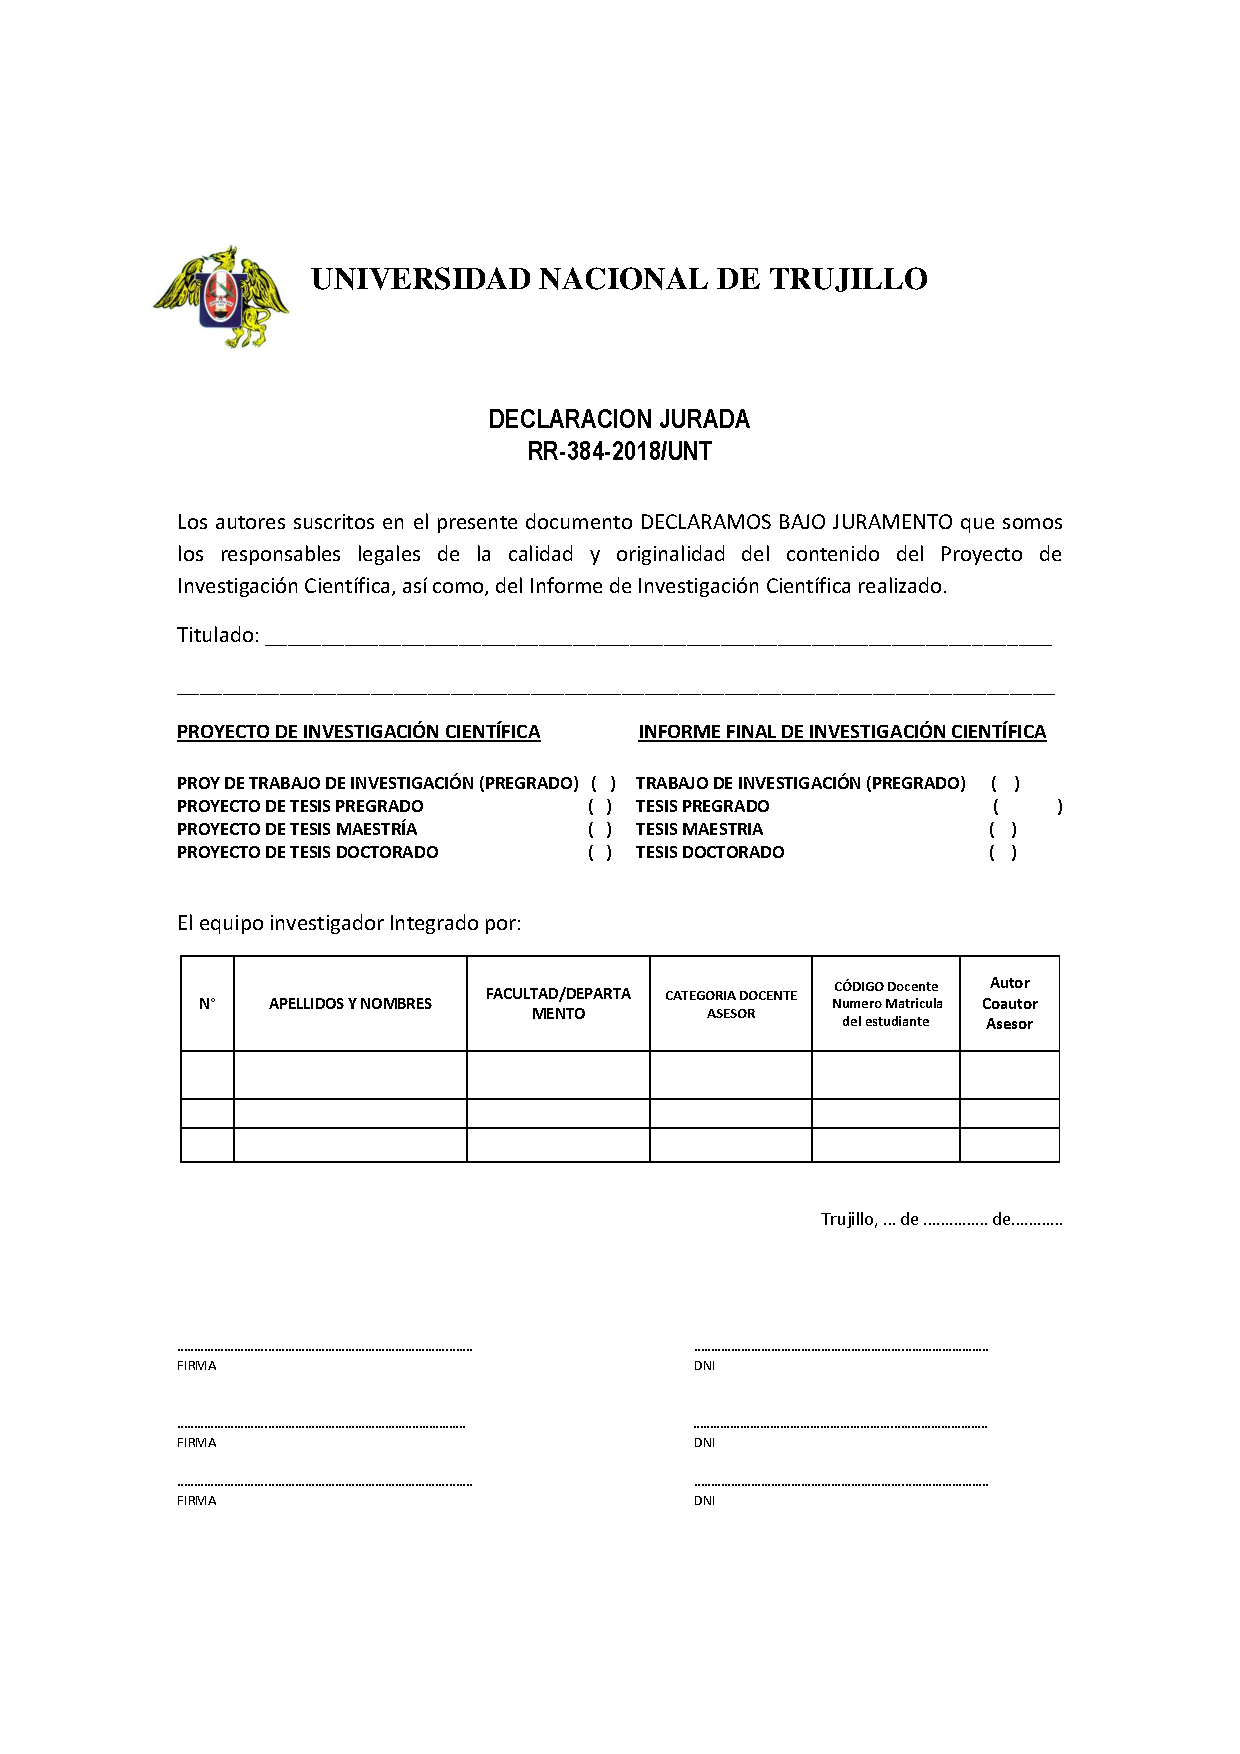
\includepdf[pagecommand={}]{DECLARACION_JURADA.pdf}
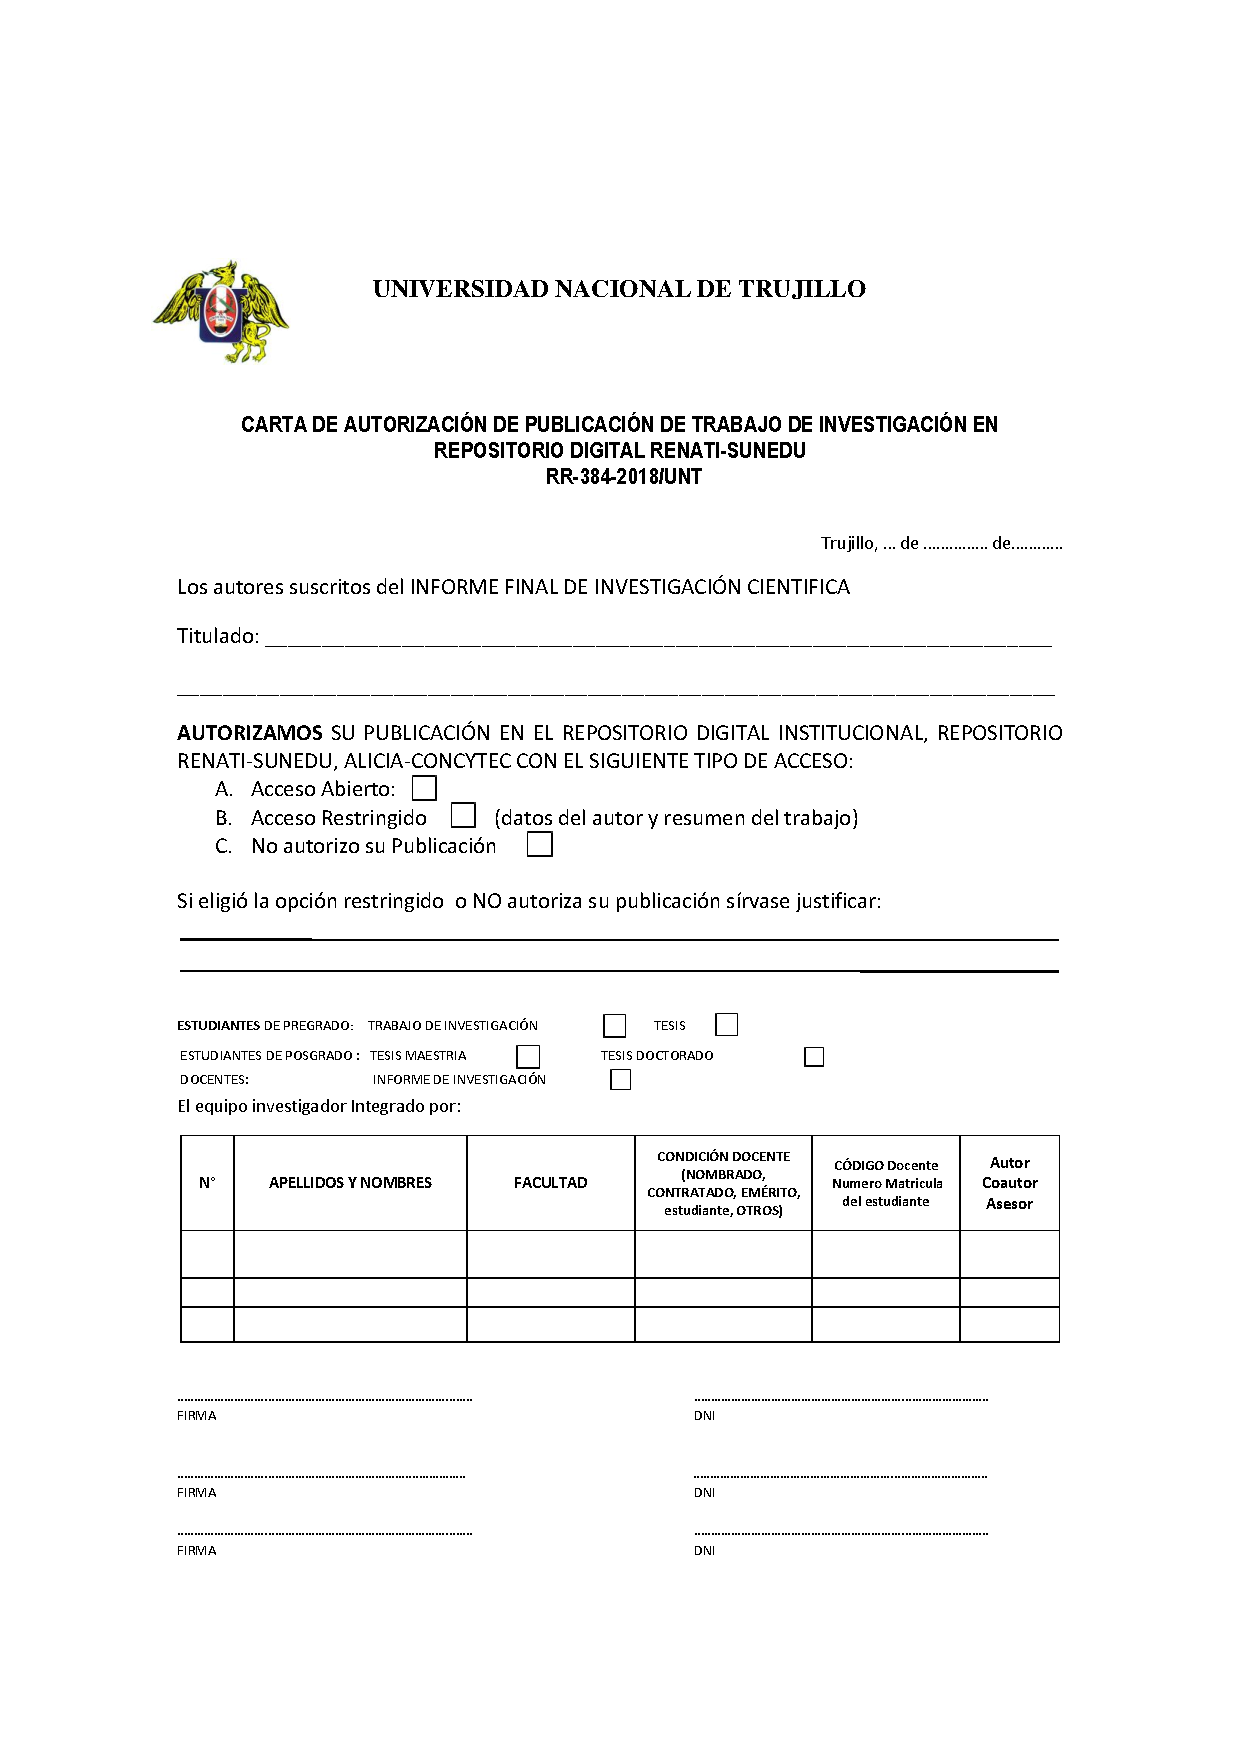
\includepdf[pagecommand={}]{CARTA_AUTORIZACION.pdf}

\end{document}






